\documentclass{article}

\usepackage[T1]{fontenc}
\usepackage[utf8]{inputenc}
\usepackage{graphicx}
\usepackage{xcolor}
\usepackage[francais]{babel}
\usepackage{tgtermes}
\usepackage{tikz-timing}
\usepackage{amsmath,amssymb,amsthm,textcomp}
\usepackage{enumerate}
\usepackage{multicol}
\usepackage{tikz}
\usepackage{tabu}
\usepackage{color}
\usepackage{adjustbox}
\usepackage{graphicx}
\renewcommand\labelenumi{(\theenumi)}
\usepackage{wrapfig}
\usepackage[hyphens]{url}
\usepackage{geometry}
\usepackage[footnotesize,labelfont=bf,hang]{caption}
\usepackage[bottom]{footmisc}
%\usepackage{biblatex}

\usepackage[
pdftitle={BigProject}, 
pdfauthor={Simon Camille},
colorlinks=true,linkcolor=blue,urlcolor=blue,citecolor=blue,bookmarks=true,
bookmarksopenlevel=2]{hyperref}

\geometry{total={210mm,297mm},
left=25mm,right=25mm,%
bindingoffset=0mm, top=20mm,bottom=20mm}

\linespread{1.3}

\newcommand{\linia}{\rule{\linewidth}{0.5pt}}
\newcommand{\oeuvre}{\oe uvre }
\newcommand{\noeud}{n\oe ud }
\newcommand{\noeuds}{n\oe uds }
\newcommand{\blap}[1]{%
\smash[b]{\begin{tabular}[t]{@{}c@{}}#1\end{tabular}}}
 
\renewcommand{\baselinestretch}{1.5}

\setlength{\parskip}{1em}

\hypersetup{breaklinks=true}

% my own titles
\makeatletter

\renewcommand{\maketitle}{
    \begin{center}
    \vspace{2ex}
    {\huge \textsc{\@title}}
    \vspace{1ex}
    \\
    \linia\\
    \@author \hfill \@date
    \vspace{4ex}
    \end{center}
}

\makeatother

%%%%%%%%%%%%%%%%%%%%%%%%%%%%%%%%%%%%%%%%%%%%%%%%%%%%%%%%%%%%%%%%%%%%%%%%%%%%

\title{La technologie Blockchain}
\author{Camille Simon}
\date{Master 2 IWOCS}

\begin{document}

\maketitle

\section*{Introduction}

Fin 2017, le cours de la monnaie virtuelle \textit{Bitcoin} s'envole. Cette étrange devise, peu connue du grand public, se retrouve à la une de tous les média. Commence alors la diffusion des termes \textit{Bitcoin}, \textit{Blockchain} et \textit{cryptomonnaies} dans le vocabulaire courant. Mais que désignent ces mots ? Dans cette introduction, nous définirons le vocabulaire essentiel.

\begin{wrapfigure}{R}{0.5\textwidth}
    \vspace{-10pt}
    \centering
    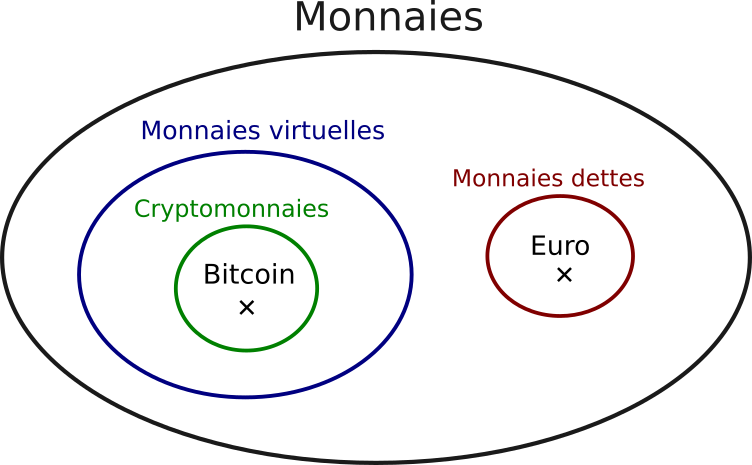
\includegraphics[width=0.48\textwidth]{schema-monnaies.png}
    \caption{Diagramme des monnaies}
    \vspace{-15pt}
\end{wrapfigure}

On appelle \textit{monnaie} une unité qui sert à exprimer le prix des objets ou des services. Le \textit{Bitcoin} est une \textit{cryptomonnaie}. Les \textit{cryptomonnaies} sont caractérisées par l'utilisation de procédés cryptographiques ainsi que par l'implication des utilisateurs dans la création et l'échange de la monnaie. Le Bitcoin fait partie des \textit{monnaies virtuelles}. Elles se différencient des monnaies que nous connaissons\footnote{Les devises utilisées par les États sont appelées \textit{monnaies dettes}. Cette appellation vient du fait que l'argent est créé par le remboursement des dettes. Plus d'informations sur les monnaies réelles ou virtuelles : \textbf{Laborde}, Stéphane (2012) \textit{La théorie relative de la monnaie}. Consultable en ligne : \url{http://trm.creationmonetaire.info/} (Consulté le 22/02/2018).}, comme l'euro, la monnaie unique de l'Union Européenne, du fait qu'elles n'ont pas de réalité physique. Si vous souhaitez acheter une baguette de pain en euro, vous pouvez le faire à l'aide de pièces ou de billets ayant une valeur fixée. Mais, ce n'est pas le cas avec la monnaie Bitcoin, car elle n'a pas de forme tangible. Les Bitcoins sont stockés sur des supports numériques (clé USB, ordinateur, smart phone,...) et échangés à travers un réseau décentralisé. De manière générale, on appelle \textit{transaction} le fait de réaliser une opération financière. Les transactions réalisées avec des Bitcoins sont consignées dans un grand "registre" public appelé \textit{Blockchain}. 

Qu'est-ce que la \textit{Blockchain} ? Quel est son principe de fonctionnement ? Est-elle indissociable de la monnaie Bitcoin ? Quels pourraient être ses domaines d'application et quelles en seraient les limites ?

Pour répondre à ces questions, le présent rapport commencera par présenter un rapide historique de la Blockchain ainsi que son fonctionnement. Suivra une présentation des différents domaines d'applications et des limites de cette technologie. Enfin, nous verrons quelles évolutions sont envisageables dans le futur pour la Blockchain.

%TODP vérifier que toutes les def essentiels sont dans l'intro

\section{Rappel historique}

La technologie Blockchain a été évoquée pour la première fois en 2008 dans un article intitulé \textit{Bitcoin: A Peer-to-Peer Electronic Cash System}\footnote{\textbf{Nakamoto}, Satoshi (2008). \textit{Bitcoin: A Peer-to-Peer Electronic Cash System}. Consultable en ligne : \url{https://bitcoin.org/bitcoin.pdf} (Consulté le 27/02/2018).} écrit par Satoshi Nakamoto. Il y présente son idée de création d'une monnaie décentralisée et dont les transactions seraient totalement transparentes. Il appelle Blockchain le support d'information enregistrant l'ensemble des transactions de façon transparente, anonyme et sécurisée.

Pendant les deux années suivantes Satoshi met en place la monnaie Bitcoin. Il crée notamment un logiciel intitulé \textit{Bitcoin-QT} permettant de créer des unités monétaires. Avec le Bitcoin, Satoshi Nakamoto essaie de mettre à l'épreuve le raisonnement qu'il a exprimé dans son article. Il choisit de reproduire le modèle des ressources naturelles finies comme les métaux. C'est-à-dire qu'il fait en sorte que les utilisateurs ne puissent produire qu'un nombre déterminé de Bitcoin.

Son expérience inspire entre 2013 et 2014 une multitude d'autres monnaies\footnote{Le site BitCoin.org a tenté de faire une liste des monnaies virtuelles : \url{https://bitcoin.fr/une-classification-des-monnaies-decentralisees/}} qui présentent des variations du modèle proposé par Satoshi. La plupart de ces monnaies continuent toutefois d'utiliser la Blockchain comme support d'information.

Le Bitcoin n'est connu que d'un petit nombre d'internautes jusqu'au mois de novembre 2017 où les spéculateurs s'en emparent. À partir de ce moment-là, le taux d'échange du Bitcoin vers les monnaies dettes explose\footnote{Le cours du Bitcoin en temps réel peut être suivi sur : \url{https://bitcoin.fr/Cours-du-bitcoin/}}. Cette hausse spectaculaire du cours du Bitcoin est due à l'intérêt grandissant des banques pour cette nouvelle devise.

Cette publicité autour du Bitcoin amène un public de plus en plus nombreux à s'intéresser au fonctionnement de la cryptomonnaie et de la Blockchain. Les entreprises se rendent alors compte du potentiel que représente la Blockchain.

%https://webusers.imj-prg.fr/~ricardo.perez-marco/BlockChain/BitcoinP7.pdf ???
%https://openclassrooms.com/courses/comprendre-le-bitcoin-et-la-BlockChain/le-principe-du-bitcoin-1-2-la-BlockChain
%https://www.meteo-BlockChain.fr/digmasbord-BlockChain/l-histoire-de-la-BlockChain/
%https://steemit.com/BlockChain/@alsaceBlockChain/BlockChain-un-peu-d-histoire-and-pourquoi-cela-fonctionne
%https://bitcoin.org/bitcoin.pdf
%https://bitcoin.fr/une-classification-des-monnaies-decentralisees/
%https://bitcoin.fr/Cours-du-bitcoin/
%\footnote{File:Hachage.svg. (2017, September 14). Wikimedia Commons, . Retrieved 08:27, février 28, 2018 from https://commons.wikimedia.org/w/index.php?title=File:Hachage.svg&oldid=258582573.}

\section{Principe \& fonctionnement}

Avant de détailler le fonctionnement de la Blockchain, il est nécessaire de définir ce qu'est une \textit{fonction de condensat} également appelé \textit{fonction de hachage}.

\subsection{Fonction de condensat}

Les fonctions de condensat sont utilisées en cryptographie et en informatique. Il s'agit de fonctions qui prennent en entrée une donnée et retournent une \textit{empreinte} ou une \textit{signature} de taille fixée, également appelée \textit{hash} qui garantit l'intégrité de cette donnée. La donnée peut être non seulement une liste de transactions comme dans le cas du Bitcoin, mais encore n'importe quel type d'information. Pour obtenir la signature d'une donnée, les fonctions de hachage les plus connues sont le \textit{MD5} et le \textit{SHA-256}. L'exemple ci-dessous présente les hash obtenus à partir de différentes chaînes de caractères en utilisant la fonction \textit{MD5}.

\begin{wrapfigure}{L}{0.48\textwidth}
    \vspace{-20pt}
    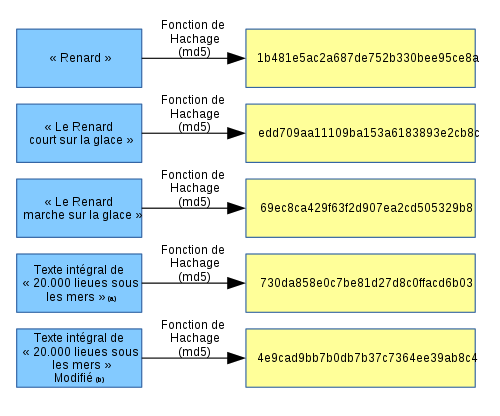
\includegraphics[width=0.48\textwidth]{500px-Hachagesvg.png}
    \caption{Exemples de hachages de textes par la fonction md5; (a) le texte utilisé est la version libre de "20.000 lieues sous les mers" du projet Gutenberg; (b) la version modifiée est le même fichier texte, le 10ème caractère de la 1000ième ligne ayant été remplacé par le caractère "*".}
    \vspace{-20pt}
\end{wrapfigure}

Les fonctions de hachage sont caractérisées par les trois propriétés suivantes : 

\begin{itemize}
    \item Il est facile d'obtenir le hash d'une information. Cette opération demande un temps de calcul négligeable.
    \item L'opération réciproque, c'est-à-dire reconstituer un document en fonction de son hash est au contraire impossible. Cette propriété est appelée "propriété de sens unique".
    
    \item On appelle \textit{collision} deux empreintes identiques provenant du hachage de deux informations différentes. Pour que la fonction de condensat soit considérée comme étant de bonne qualité, il faut qu'elle limite le nombre de collision. Cette propriété est dite de "résistance aux collisions". 
\end{itemize}

On supposera dans la suite du document que le hash d'une information est unique. Passons maintenant à la description de la structure Blockchain.

\subsection{Description de la structure Blockchain}

Commençons par nous intéresser à l'élément central d'une Blockchain, le bloc. Tous les blocs de la Blockchain comportent les éléments suivants : un \textit{index}, une date de création \textit{timestamp}, de l'information \textit{data}, le hash du bloc précédent dans la Blockchain \textit{previousHash}, et le \textit{hash} de son propre bloc. Détaillons ces différents éléments.

\subsubsection*{Index}

L'\textit{index} est un numéro indiquant l'emplacement du bloc dans la liste. Le bloc d'index 0 est le premier bloc de la chaîne. Le bloc d'index 8 est le 9\textsuperscript{ème} bloc de la chaîne, et de manière générale le bloc d'index $i$ est donc le $i+1$\textsuperscript{ème} bloc de la chaîne.

\subsubsection*{Timestamp}

Le \textit{timestamp}, également appelé horodatage en français, sert à renseigner le moment où le bloc commence à être créé. Il existe plusieurs formats de temps. Dans le cas du Bitcoin, c'est le format de temps POSIX, très répandu en informatique, qui a été choisi. Il s'agit du nombre de secondes écoulées depuis le 1\textsuperscript{er} janvier 1970 à minuit au méridien de Greenwich. Pour une lecture du temps plus aisée, on peut choisir le standard ISO 8601. Voici un exemple de ces deux formats de temps :
\begin{center}
    \vspace{-15pt}
    POSIX : $1519398019$ \\
    ISO 8601: $2018-02-23T15:00:19Z$
\end{center}

%https://fr.wikipedia.org/wiki/Blockchain
%https://fr.wikipedia.org/wiki/R%C3%A9seau
%https://fr.wikipedia.org/wiki/Horodatage
%https://fr.wikipedia.org/wiki/Date_(m%C3%A9tadonn%C3%A9e)
%https://fr.wikipedia.org/wiki/Heure_Unix
%https://fr.wikipedia.org/wiki/Temps_universel_coordonn%C3%A9#UTC_et_GMT

\subsubsection*{Data}

Il est possible d'enregistrer dans la Blockchain des informations de toutes sortes : des transactions, des messages, des enregistrements semblables à ce que l'on peut trouver dans des bases de données ou encore des URL. Cette information est appelée \textit{data} du bloc. Elle peut être en partie ou entièrement chiffrée\footnote{Le terme "crypter" n'est pas un mot de la langue française, bien qu'il soit reconnu au Québec. Plus d'informations sur le bon emploi de ces termes sur : \url{https://chiffrer.info/}.} afin de la sécuriser.

%https://marmelab.com/blog/2016/05/12/blockchain-expliquee-aux-developpeurs-web-la-theorie.html
%https://medium.com/@lhartikk/a-blockchain-in-200-lines-of-code-963cc1cc0e54
%https://www.ibm.com/developerworks/library/j-chaincode-for-java-developers/index.html
%https://www.ssaurel.com/blog/create-your-own-blockchain-in-30-minutes/

\subsubsection*{Hash et previousHash}

Le \textit{hash} du bloc est le résultat de la fonction de condensat ayant pris en entrée l'index, le \textit{timestamp}, le \textit{previousHash} et les données du bloc. Le \textit{previousHash} quant à lui fait référence au \textit{hash} du bloc précédent dans la chaîne. 

Une fois le \textit{hash} calculé il n'est plus possible de modifier l'index, le \textit{previousHash}, le \textit{timestamp} ou les données. Une modification, même infime, de leurs contenus entraînerai la génération d'un \textit{hash} différent. C'est cette propriété qui assure l'intégrité du bloc. Pour s'assurer qu'un bloc n'est pas corrompu, il suffit de vérifier que son \textit{hash} est égal au résultat de la fonction de condensat des éléments du bloc. 

De plus, le \textit{previousHash} est une donnée utilisée dans la génération du \textit{hash}. De cette façon on scelle le lien entre le bloc et son prédécesseur, créant ainsi une Blockchain, une chaîne de blocs ordonnés.

\begin{figure}[!h]
    \centering
    \vspace{20pt}
    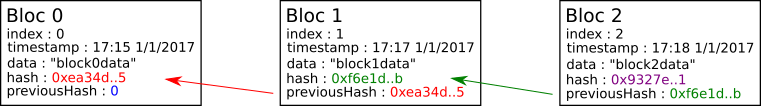
\includegraphics[scale=0.7]{blockchain.png}
    \caption{Chaîne de blocs.}
    \label{fig:my_label}
\end{figure}

%Si on souhaite intercaler un nouveau Block, il est nécessaire de recalculer le hash de son suivant qui doit modifier son previsouHash. Ces modifications se reporte sur tous les Blocks suivant de la chaîne. Le même processus se produit si l'on souhaite modifier un Block existant.

%\begin{figure}[!h]
%    \centering
%    \vspace{5pt}
%    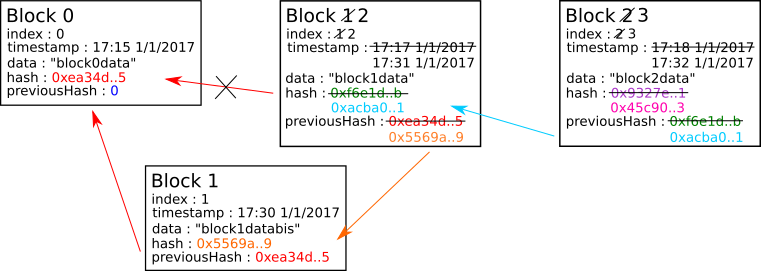
\includegraphics[scale=0.7]{blockchain-modif.png}
%    \caption{Ajout d'un Block en 2\textsuperscript{ème} place dans la chaîne.}
%    \label{fig:my_label}
%    \vspace{-5pt}
%\end{figure}

%https://medium.com/@lhartikk/a-blockchain-in-200-lines-of-code-963cc1cc0e54

%Il existe trois types de Blockchain : 
%\begin{description}
%    \item[Les Blockchain publiques] où l'accès n'est pas restreint, tout le monde peut devenir un noeud du réseau
%    \item Les Blockchain privée où l'accès au réseau est contrôlé
%    \item Les Blockchain mixtes
%\end{description}

\subsection{Mise en \oeuvre de la Blockchain}

On appelle \textit{réseau} un ensemble de \textit{\noeuds}reliés ensembles et communicant entre eux. Chaque \noeud possède une copie de la Blockchain. Un \noeud peut être un ordinateur ou un groupe d'ordinateurs. Lorsqu'un nouveau \noeud rejoint le réseau, il reçoit une copie de la Blockchain. L'ensemble des \noeuds qui produisent les nouveaux blocs sont appelés \textit{mineurs} et le processus de création se nomme \textit{le minage}.

On distingue trois types de Blockchain. Elles se différencient en fonction de l'attribution du droit de minage : 
\begin{itemize}
    \item Dans les \textit{Blockchain publiques}, tout le monde peut devenir un \noeud du réseau et un mineur, il n'y a aucune restriction.
    \item Dans les \textit{Blockchain privées}, il faut une première autorisation pour devenir un \noeud du réseau et une deuxième pour devenir un mineur.
    \item Il existe enfin des \textit{Blockchain hybrides} qui allient les aspects publics et privés.
\end{itemize}

\subsubsection{Principe du Minage}

Chaque mineur construit un bloc dit \textit{local}, c'est-à-dire qu'il construit un bloc à partir des informations dont il a connaissance. Dans le cas du Bitcoin, chaque mineur enregistre les transactions dans l'ordre dans lequel elles lui parviennent. Cet ordre peut être différent d'un mineur à l'autre. On peut généraliser en appelant \textit{faits} les informations transitant sur le réseau et collectées par les mineurs.

Reste maintenant à établir quel bloc local va devenir le nouveau bloc de la Blockchain. Il existe différents types de \textit{consensus} également appelés \textit{preuve}. Sur le schéma ci-dessous, le nouveau bloc est choisi de façon aléatoire. Chaque mineur lance une paire de dés, on relance les dés jusqu'à ce que l'un des mineurs obtienne un double six. C'est alors son bloc qui est choisi pour être ajouté à la Blockchain.

\begin{figure}[!h]
    \centering
    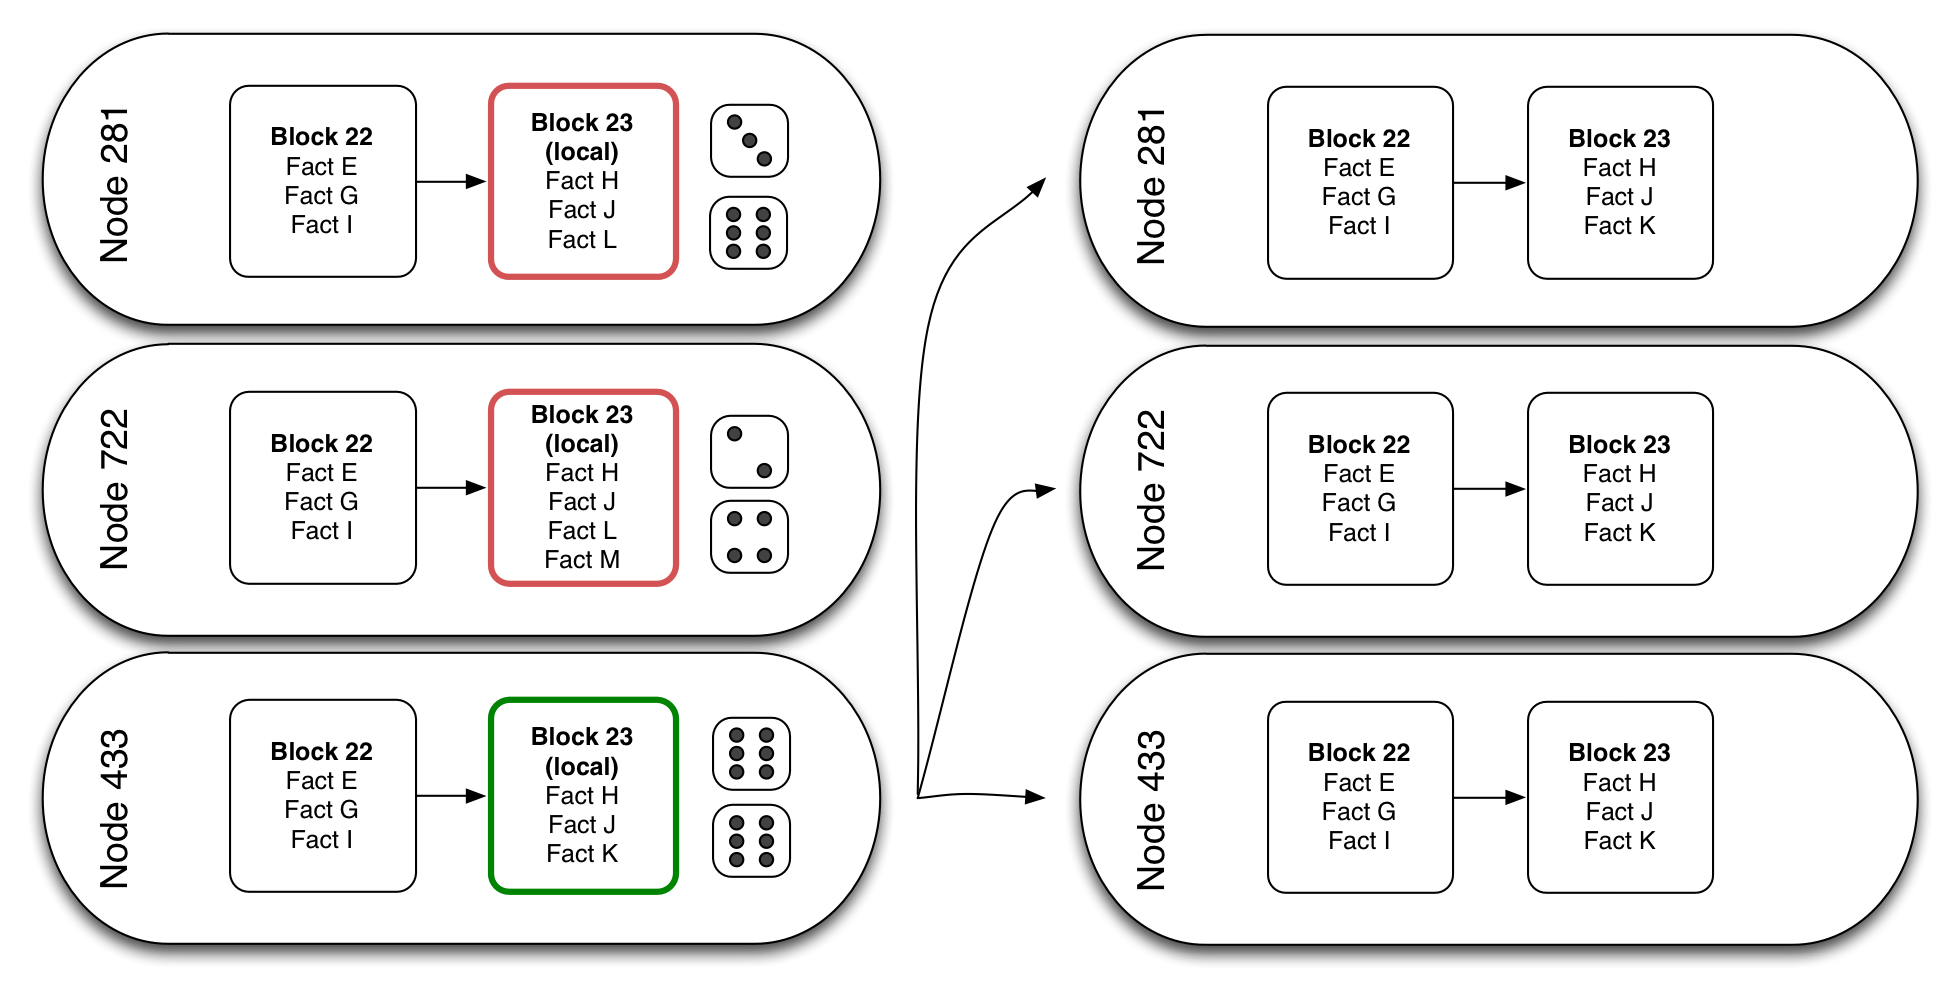
\includegraphics[scale=0.46]{rolling_dice.png}
    \caption{Le mineur obtenant un double six obtient le droit de diffuser son bloc local qui devient le nouveau bloc de la Blockchain.}
    \vspace{-10pt}
    \label{fig:my_label}
\end{figure}

Il existe différentes types preuves : 

\begin{itemize}
    \item La \textit{preuve d'autorité}, également appelé \textit{proof of authority}, consiste à ne donner le droit de miner qu'à un petit groupe de \noeuds ayant la confiance du réseau. Cette méthode est majoritairement employée dans les Blockchains privées.
    \item La \textit{preuve de travail}, appelé \textit{proof of work} en anglais, est la plus répandue. Elle consiste à demander aux mineurs qui souhaitent soumettre un bloc de résoudre un problème non seulement long et difficile, mais encore nécessitant une puissance de calcul importante. Le premier mineur qui résout l'énigme voit son bloc sélectionné pour être le nouveau bloc de la Blockchain. Dans le cas du Bitcoin, on demande aux mineurs de générer un \textit{hash} commençant par un nombre donné de zéros. Il est nécessaire de hacher un grand nombre de chaîne de caractères avant de trouver un \textit{hash} valide. Cette preuve est très utilisée dans les Blockchains publiques.
    \item La \textit{preuve d'enjeu}, \textit{proof of stake}, se présente comme une alternative à la preuve de travail. Les mineurs disposent de jetons qu'ils peuvent mettre en dépôt, lors du consensus, l'un des jetons du dépôt est choisi aléatoirement, c'est le mineur auquel il appartient qui doit produire le prochain bloc. S'il ne produit pas le bloc dans le temps imparti, c'est un autre jeton qui est sélectionné. Un mineur peut augmenter ses chances d'être sélectionné en déposant un grand nombre de jetons. Cette preuve est de plus en plus usitée dans les Blockchains publiques.
\end{itemize}

%Les faits non sélectionnés ?

Bien sûr, il existe d'autres preuves : des preuves aléatoires comme celle présentée sur la figure 4 ou des preuves sélectionnant le bloc de longueur maximale.

\subsubsection{Validation de la chaîne}

%Réception Block => vérification

Les \noeuds sont amenés à vérifier l'intégrité de leur Blockchain. Il y a deux vérifications à effectuer : une première afin de s'assurer que la Blockchain n'a pas été modifiée localement et une seconde s'assurant que tous les \noeuds disposent de la même Blockchain.

\textbf{Vérification locale}

À la réception d'un nouveau bloc, chaque \noeud doit vérifier que l'intégrité du bloc reçu n'a pas été altérée. Pour ce faire, on calcule le hash du bloc via la fonction de condensat, et on compare l'empreinte obtenue avec l'empreinte attachée au bloc. Si elles sont identiques, le \noeud peut ajouter le bloc à sa Blockchain; en revanche, si une anomalie est détectée, le \noeud doit demander à un autre \noeud du réseau de lui renvoyer le bloc.

À intervalles de temps réguliers, les \noeuds doivent également vérifier que l'intégralité de leur chaîne est correcte. On vérifie alors chaque bloc de la même manière que pour les nouveaux blocs à ajouter en partant du dernier bloc et en remontant la chaîne via le \textit{previousHash}. S’il y a un ou plusieurs blocs corrompus, le \noeud demande à un des autres \noeuds du réseau de lui renvoyer la Blockchain à partir du bloc non fiable le plus ancien. % le plus haut dans la liste ?.

\newpage

%https://www.technologies-ebusiness.com/enjeux-et-tendances/benefices-de-preuve-dautorite-proof-of-authority-poa
%https://www.ethereum-france.com/quest-ce-que-la-preuve-denjeu-proof-of-stake-faq-par-v-buterin-traduction-francaise/
%http://karlodwyer.com/publications/pdf/bitcoin_KJOD_2014.pdf
%https://fr.wikipedia.org/wiki/Attaque_Sybil

\textbf{Vérification à l'échelle du réseau}

La Blockchain doit être unique, elle doit donc être la même sur l'ensemble des \noeuds du réseau. S’il y a plusieurs Blockchains sur le réseau, la Blockchain la plus répandue sera considérée comme la Blockchain légitime. Les \noeuds non conformes devront donc la récupérer afin qu'il n'y ait qu'une unique Blockchain partagée par tous les \noeuds.

\section{Domaines d'application}

Les domaines d'applications de la Blockchain sont variés : banque, finance, assurance, logistique, industrie, énergie, etc. Cependant, il ne s'agit que de déclinaisons de deux grands types d'applications : l'utilisation de la Blockchain comme un registre d'information d'une part et comme remplacement des tiers de confiance d'autre part.

\subsection{Registre}

Le premier usage que l'on trouve à la Blockchain est celui pour lequel elle a été conçue : enregistrer de l'information de façon pérenne. En effet, la structure en liste ordonnée dans le temps permet de stocker les informations de façon chronologique. On peut donc utiliser la Blockchain pour toutes les applications du type registre, par exemple registres d'état civil, registres matrimoniaux, registres des naissances, lois, etc.
Par extension, elle peut également garder trace des transactions ou transferts d'informations, par exemple pour les registres bancaires et financiers, registres de bibliothèques, etc.

%Pérennité => papier description
%Registre d'état civil => naissance & décès

\subsection{Smart Contrat}

La deuxième grande famille d'applications, moins connue, mais très prometteuse, consiste à utiliser la Blockchain comme un Smart Contrat. 

Étudions un cas concret : un propriétaire met en location un logement au prix de 1 000 € par semaine. Un premier versement de 50 \% de la somme se fait à la réservation du logement. Le locataire doit également donner un chèque de caution de 5 000 €. Les 50 \% restant seront versés à la fin de la location. Tous ces éléments sont inscrits dans un contrat signé par le locataire et le propriétaire.

Malheureusement, à la fin de la location le locataire refuse de verser les 50 \% restant. De plus, une vitre a été cassée, et lorsque le propriétaire a voulu encaisser le chèque, celui-ci a été refusé car le compte était vide. Le propriétaire décide donc de porter plainte et comparait au tribunal. Les acteurs en présence sont donc les suivants : le propriétaire, le locataire, le juriste qui a rédigé le contrat de location, la banque maniant les fonds, l'avocat et le tribunal pour la plainte.

Dans le cas d'un Smart Contrat, les différents éléments du contrat sont enregistrés sous la forme de mini-programmes dans des blocs. Les deux parties, locataire et propriétaire, scellent le contrat ensemble de façon à ce qu’eux seuls puissent l'annuler\footnote{Il s'agit d'un mécanisme de clé publique/clé privé qui n'est pas présenté ici car il n'est pas utilisé dans toutes les Blockchains. Vous pouvez consulter une rapide présentation à l'adresse suivante : \url{http://www-igm.univ-mlv.fr/~dr/XPOSE2006/depail/fonctionnement.html}}. Le mini-programme s'exécute à un moment donné par un horodatage inscrit dans le bloc. 

\vspace{1em}

Dans notre cas cela donnerait :
\begin{itemize}
    \item Un premier bloc effectuant le virement de 50 \% de la somme du locataire vers le propriétaire, et la mise en place d'un verrou sur le reste de la somme. Ce bloc s'exécute deux semaines avant la location.
    \item Le deuxième bloc ne s'exécute que si la location est annulée avant la date de début de location. Il fait le virement des 50 \% du propriétaire vers le locataire et lève le verrou sur l'argent du locataire. Il annule également la suite du contrat.
    \item Le troisième bloc se déclenche à la date de début de la location et verrouille les 5 000 € de caution.
    \item À la fin de la location, le quatrième bloc effectue le virement des 50 \% restant du locataire vers le propriétaire.
    \item Reste maintenant à libérer la caution, cela ne peut se faire que si les deux parties sont d'accord. S’il y a eu dégradation, c'est le cinquième bloc qui s'exécute et vire la caution au propriétaire. Sinon, c'est le sixième bloc qui s'exécute, il enlève le verrou sur l'argent réservé pour la caution.
    \item Le contrat continu d'exister tant que la Blockchain existe. 
\end{itemize}

\vspace{1em}

Dans le cas de l'usage d'une Blockchain, il devient possible de réduire les intermédiaires comme les juristes. De plus, ce type de contrat peut remplacer les \textit{tiers de confiance} comme les banques qui servent habituellement de garants afin de verrouiller les fonds le temps de la transaction.

%\subsection{}

%\subsubsection*{Les banques}

%Comme nous l'avons vu avec le Bitcoin ou avec les Smart Contrats, la Blockchain peut remplacer les banques. A une époque où il ne s'écoule pas une année sans la révélation d'un scandale financier, l'opportunité d'avoir accès à un registre des comptes infalsifiable et public permettrait de vérifier aisément à quelles fins l'argent est dépensé.

%Une quarantaine de banques ont pour l'heure décider de travailler ensemble ainsi qu'avec l'entreprise R3 CEV afin d'établir des standards pour les Blockchains aux seins des banques. Le but étant de copier le principe des cryptomonnaies afin de l'appliquer pour les monnaies-dettes.


\section{Limites et perspectives}

%http://assistance.bitconseil.fr/support/solutions/articles/31000135176-taille-et-emplacement-de-la-blockchain-de-bitcoin
Une première limite concerne la taille de la Blockchain. En effet, comme la Blockchain doit être unique, toutes les informations sont enregistrées dans la même liste. On estime la taille actuelle de la Blockchain utilisée pour les transactions Bitcoin à 150 Go\footnote{Il est possible de suivre en temps réel l'évolution de la taille de la Blockchain sur : \url{https://charts.bitcoin.com/chart/blockchain-size}}. Cette taille importante impose aux \noeuds du réseau de disposer de suffisamment d'espace mémoire. Toutefois, ceci peut être nuancé aux vues du faible coût de l'espace mémoire. Cette contrainte est plus importante dans le cas d'une application aux objets connectés où les ressources sont plus restreintes.

En fonction du nombre de \noeuds sur le réseau, certains problèmes peuvent émerger. Une fois le consensus réalisé, le nouveau bloc élu doit être envoyé à l'ensemble des \noeuds ce qui engendre un encombrement du réseau. De plus, les mineurs ne peuvent proposer de nouveaux blocs qu'une fois le bloc précédent réceptionné par l'ensemble des \noeuds. Cette attente des \noeuds se traduit par des effets de latence sur le réseau. Le phénomène de latence augmente davantage lorsque qu'une partie de la Blockchain doit transiter entre les \noeuds. C'est le cas si un ensemble de \noeuds n'a pas la bonne version de la Blockchain. 

%https://halshs.archives-ouvertes.fr/halshs-01673329/file/17057.pdf
%http://data.em-lyon.com/wp-content/uploads/2017/01/GODEBARGE_ROSSAT_Blockchain-version-finale.pdf
%http://www.agoravox.fr/actualites/economie/article/les-cryptomonnaies-du-futur-189712
%https://www.fournisseur-energie.com/monnaies-numeriques-impact-ecologique/

Beaucoup de détracteurs de la Blockchain lui reprochent son coût énergétique. Il s'agit là d'un double amalgame. En effet ce n'est pas la Blockchain en elle-même qui nécessite beaucoup de ressource, c'est éventuellement la preuve de travail. Il s'agit en réalité plus d'un problème propre aux cryptomonnaies car la difficulté de la preuve de travail est augmentée régulièrement. Cette augmentation de la difficulté entraîne la consommation de ressources machines toujours plus importantes. Il est possible d'utiliser la preuve de travail sans connaître de coût énergétique excessif. De même, il existe d'autres preuves pouvant être adoptées. Il suffit de prendre pour exemple la monnaie virtuelle \textit{Ğ1} dont l'impact carbone est très faible car ce n'est pas le minage qui génère la création de monnaie\footnote{La description de la monnaie \textit{Ğ1} ainsi que son mode de fonctionnement sont décrit à l'adresse : \url{https://duniter.org/fr/duniter-pourquoi-comment/}.}. 

%https://bitconnect.co/bitcoin-news/119/top-5-blockchain-technology-myths-the-mainstream-has-fallen-for

%- Taille de la Blockchain
%- Sur le réseau : scalability and latency issues
%- Le type de consensus a beaucoup d'importance
%- Réécriture de la Blockchain => limite des usages
%Perspectives :
%Holochain

\clearpage

\section*{Conclusion}

La technologie Blockchain a été créée en 2008 en même temps que la cryptomonnaie Bitcoin. Elle a été conçue afin de servir de registre aux transactions financières de façon à ce que l'information soit décentralisée, sécurisée et anonyme. Concrètement mise en place à partir de 2013, cette première Blockchain est toujours en activité.

L'intérêt des banques pour cette nouvelle économie a également mis en lumière la technologie sous-jacente : la Blockchain. Dès lors, les entreprises ont commencé à vouloir exploiter cette technologie dans de multiples domaines d'autant plus qu'elle est facile à mettre en \oeuvre.

Quoique simple, le structure en chaîne de bloc suffit néanmoins à garantir la sécurité et l'intégrité des données. De plus, la Blockchain est répliquée sur l'ensemble des \noeuds du réseau assurant ainsi sa robustesse.

Il existe trois types de Blockchain en fonction des droits de minage, de la plus restrictive, la Blockchain privée à la plus permissive, le Blockchain publique. Quel que soit le type de Blockchain, le choix de la preuve influe sur la dépense énergétique et la latence du réseau. Seules quelques limites sont connues à la Blockchain notamment sa taille en constante augmentation et l'encombrement du réseau proportionnel à cette taille.

%Qu'est-ce que la \textit{Blockchain} ? Quel est son principe de fonctionnement ? Est-elle indissociable de la monnaie Bitcoin ? Quels pourraient être ses domaines d'application et quelles en seraient les limites ?

Cette technologie, relativement récente, est pour l'heure peu documentée. La Blockchain est aujourd'hui presque intégralement déployée dans le domaine des cryptomonnaies, pourtant il existe de multiples domaines d'applications à cette technologie. Nous ne sommes aujourd'hui qu'à l'aube de l'avènement de la Blockchain qui devrait révolutionner notre façon de le fiabiliser les transactions numériques.

%un peu plus nous menez vers une société tout numérique. %

\clearpage

\section*{Bibliographie}

2016, GODEBARGE Ferréol, ROSSAT R, et Godebarge Ferréol, Rossat Romain. «Principes clés d’une application blockchain», 15 décembre 2016. \url{http://data.em-lyon.com/wp-content/uploads/2017/01/GODEBARGE_ROSSAT_Blockchain-version-finale.pdf}.

«Attaque Sybil». \textit{Wikipédia}, 19 mai 2017. \url{https://fr.wikipedia.org/w/index.php?title=Attaque_Sybil&oldid=137477672}.

Axiaman. «Les cryptomonnaies du futur». AgoraVox, 15 février 2017. \url{http://www.agoravox.fr/actualites/economie/article/les-cryptomonnaies-du-futur-189712}.

Bitcoin. «Une classification des monnaies décentralisées – Bitcoin.fr». Bitcoin.fr, 10 février 2015. \url{https://bitcoin.fr/une-classification-des-monnaies-decentralisees/}.

«Bitcoin.Com». Consulté le 5 mars 2018. \url{https://charts.bitcoin.com/chart/blockchain-size}.

Bitconnect.co. «Top 5 Blockchain Technology Myths the Mainstream Has Fallen For | Bitconnect». Bitconnect.co. Consulté le 5 mars 2018. \url{https://bitconnect.co/bitcoin-news/119/top-5-blockchain-technology-myths-the-mainstream-has-fallen-for}.

«Blockchain». \textit{Wikipédia}, 4 mars 2018. \url{https://fr.wikipedia.org/w/index.php?title=Blockchain&oldid=146072437}.

Chateauneuf, Alain, Caroline Ventura, Alain Chateauneuf, et Caroline Ventura. \textit{Blockchain publique et contrats intelligents (Smart Contrats). Les possibilités ouvertes par Ethéreum... et ses limites}, 2009.

«Cours du bitcoin». Bitcoin.fr (blog), 8 mai 2013. https://bitcoin.fr/cours-du-bitcoin/.
«Date (métadonnée)». \textit{Wikipédia}, 31 octobre 2015. \url{https://fr.wikipedia.org/w/index.php?title=Date_(m\%C3\%A9tadonn\%C3\%A9e)&oldid=120037210}.

Dernière, Alsace blockchain dans Blockchain • L’année. «Blockchain - Un Peu d’histoire». Steemit, 24 octobre 2016. \url{https://steemit.com/blockchain/@alsaceblockchain/blockchain-un-peu-d-histoire-and-pourquoi-cela-fonctionne}.

«Fonction de hachage». \textit{Wikipédia}, 21 décembre 2017. \url{https://fr.wikipedia.org/w/index.php?title=Fonction_de_hachage&oldid=143729531}.

France, Ethereum. «Qu’est-ce que la preuve d’enjeu / Proof-of-Stake ? – FAQ par V. Buterin – Traduction française». Ethereum France, 3 janvier 2017. \url{https://www.ethereum-france.com/quest-ce-que-la-preuve-denjeu-proof-of-stake-faq-par-v-buterin-traduction-francaise/}.

Hartikka, Lauri. «A blockchain in 200 lines of code». Lauri Hartikka (blog), 4 mars 2017. \url{https://medium.com/@lhartikk/a-blockchain-in-200-lines-of-code-963cc1cc0e54}.

«Heure Unix». \textit{Wikipédia}, 18 novembre 2017. \url{https://fr.wikipedia.org/w/index.php?title=Heure_Unix&oldid=142728819}.

«Horodatage». \textit{Wikipédia}, 28 octobre 2016. \url{https://fr.wikipedia.org/w/index.php?title=Horodatage&oldid=131149114}.

inso. «Duniter, pourquoi, comment ?» Duniter, 24 janvier 2018. \url{https://duniter.org/fr/duniter-pourquoi-comment}.

J. Steven Perry. «Chaincode for Java Developers». IBM, 30 mars 2017. \url{http://www.ibm.com/developerworks/library/j-chaincode-for-java-developers/index.html}.

Karl J. O’Dwyer, David Malone. «Bitcoin Mining and its Energy Footprint». Hamilton Institute National University of Ireland Maynooth, 26 juin 2014. \url{http://karlodwyer.com/publications/pdf/bitcoin_KJOD_2014.pdf}.

«La signature numérique - Fonctionnement». Consulté le 5 mars 2018. \url{http://www-igm.univ-mlv.fr/~dr/XPOSE2006/depail/fonctionnement.htm}l.

Laborde, Stéphane. Théorie Relative de la Monnaie v2.718, 2012. \url{http://trm.creationmonetaire.info/}.

Laurent, Charlotte. «7 applications possibles de la technologie blockchain». 7x7. Consulté le 5 mars 2018. \url{https://www.7x7.press/7-applications-possibles-de-la-technologie-blockchain}.

«Les monnaies numériques et leur impact écologique». Fournisseur-Energie (blog), 20 décembre 2017. \url{https://www.fournisseur-energie.com/monnaies-numeriques-impact-ecologique/}.

Maxence. «Chiffrer.info». Chiffrer.info, 21 juillet 2016. \url{https://chiffrer.info/}.

Nakamoto, Satoshi. «Bitcoin: A Peer-to-Peer Electronic Cash System», 2008. \url{https://bitcoin.org/bitcoin.pdf}.

Rédaction Reuters. «Des transactions en “blockchain” testées par 40 grandes banques». Reuters, 3 mars 2016. \url{https://fr.reuters.com/article/companyNews/idFRL8N16B2DR}.

«Réseau». \textit{Wikipédia}, 31 janvier 2018. \url{https://fr.wikipedia.org/w/index.php?title=R\%C3\%A9seau&oldid=145050872}.

S. Saurel. «Create Your Own Blockchain in 30 Minutes – All for Android, Android for All», 27 janvier 2018. \url{https://www.ssaurel.com/blog/create-your-own-blockchain-in-30-minutes/}.

SQLI. «Les bénéfices de la Preuve d’Autorité - Proof-of-Authority (PoA)». Technologies e-business, 11 avril 2017. \url{https://www.technologies-ebusiness.com/enjeux-et-tendances/benefices-de-preuve-dautorite-proof-of-authority-poa}.

«Temps universel coordonné». \textit{Wikipédia}, 5 novembre 2017. \url{https://fr.wikipedia.org/w/index.php?title=Temps_universel_coordonn\%C3\%A9&oldid=142318935}.

webadmin. «Digmasbord raconte l’histoire de la blockchain Part1». Projet Digmasbord (blog), 24 février 2018. \url{https://www.meteo-blockchain.fr/digmasbord-blockchain/l-histoire-de-la-blockchain/}.

Zaninotto, François. «La blockchain expliquée aux développeurs web, partie 1: la théorie». Consulté le 5 mars 2018. \url{https://marmelab.com/blog/2016/05/12/blockchain-expliquee-aux-developpeurs-web-la-theorie.html}.


\end{document}

%idée d'implémentation :
%- ssd => lire/écrire/executer le + vite possible OU ram importante
%- monter dans le /tmp
